%======================================================================
\section{Study 2: why the first-order estimates fail}
\label{sec:study2}

Unless stated otherwise, results are means over the \NConfModels{} confirmation models at full strength, with 95\% bootstrap intervals over models. Study 2 recomputed the reference from its own derivatives, and it equals Study 1's saved model-level values (\RefCheckValues{} values, largest difference \RefCheckMax{}): its error ratio, the mean over models of each model's ratio of the two errors, is \RatioRefFull{} \RatioCIRefFull{}, and the mean absolute errors themselves are those of \cref{sec:effects}, \MaeFOFull{} for the reference and \MaeZeroFull{} for predicting zero change.

\subsection{Only mean replacement improves on the reference}
\label{sec:arms}

\Cref{tab:arms} and \cref{fig:ratios} give the three arms. \textbf{Mean replacement (arm~a)} lowers the error ratio to \RatioAFull{} \RatioCIAFull{}, a change of \ChangeAFull{} \ChangeCIAFull{}; it is lower than the reference in \LowerThanRefA{} of \NConfModels{} models (\cref{fig:models}). Its effects are smaller (predicting zero change has a mean absolute error of \MaeZeroAFull{} against \MaeZeroRefFull{} under silencing), and at full strength its estimate is still not distinguishable from predicting zero change (difference in mean absolute error \MaeDiffAFull{}, \MaeDiffCIAFull{}). At half strength it beats it, with an error ratio of \RatioAHalf{} \RatioCIAHalf{} (difference \MaeDiffAHalf{}, \MaeDiffCIAHalf{}). Its estimates are biased upwards (\BiasAFull{}, \BiasCIAFull{}) and give more wrong signs than the reference (\WrongAFull\%; change \WrongChangeAFull{}, \WrongChangeCIAFull{}). They still pick out the influential cell types better than anatomy (top-10 precision \TopTenAFull{} against \AnatAFull{}).

\begin{table}[t]
\centering
\caption{The reference and the three arms of Study 2. Error ratio: mean absolute error divided by that of predicting zero change on the same cases (below 1 is better than predicting zero change). Change: paired difference in error ratio from the reference. Against zero change: decision on the interval for the difference in mean absolute error. Wrong signs: fraction of large effects estimated with the opposite sign. Top-10: precision of the ten largest estimates, with anatomy (three synaptic steps) on the same cases in brackets. Means over \NConfModels{} models with 95\% bootstrap intervals.}
\label{tab:arms}
\footnotesize
\setlength{\tabcolsep}{3pt}
\begin{tabular}{@{}llllllll@{}}
\toprule
Estimate & $s$ & Error ratio & Change & \makecell[l]{Against\\ zero change} & \makecell[l]{Signed\\ error} & \makecell[l]{Wrong\\ signs} & \makecell[l]{Top-10\\ (anatomy)} \\
\midrule
\tableinput{generated/s2-table-arms.tex}
\bottomrule
\end{tabular}
\end{table}

\begin{figure}[t]
\centering
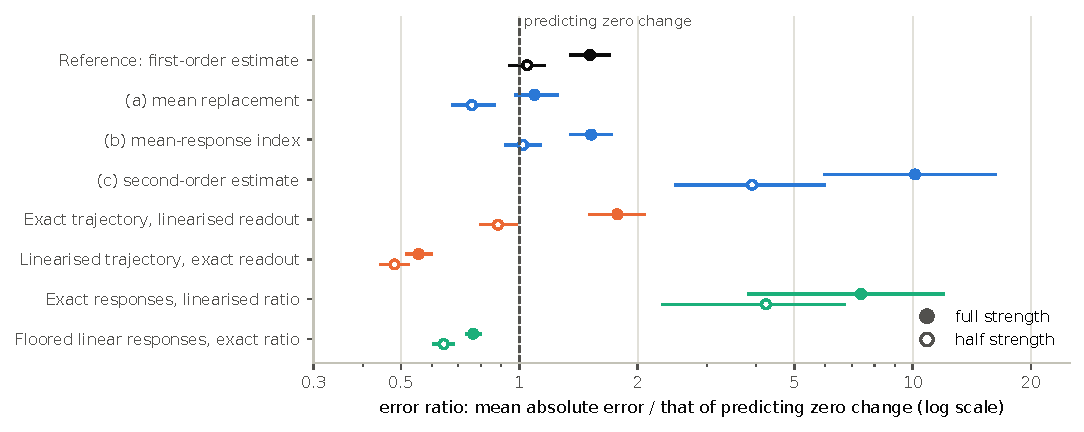
\includegraphics[width=\linewidth]{figures/s2-fig1-error-ratios.pdf}
\caption{Error ratio of every estimator of Study 2 in the \NConfModels{} confirmation models, at full strength (filled) and half strength (open), with 95\% bootstrap intervals over models. Black: the reference, Study 1's first-order estimate. Blue: the three arms, each changing one thing. Orange: the exact readout applied to the linearised trajectory, and the linearised readout applied to the exact trajectory. Green: the two stages of the readout, one exact and one linearised, on the linearised trajectory.}
\label{fig:ratios}
\end{figure}

\textbf{The mean-response index (arm~b)} changes nothing detectable: error ratio \RatioBFull{} \RatioCIBFull{}, change \ChangeBFull{} \ChangeCIBFull{}, and its estimate is worse than predicting zero change (\MaeDiffBFull{}, \MaeDiffCIBFull{}). It gives fewer wrong signs (\WrongBFull\%; change \WrongChangeBFull{}, \WrongChangeCIBFull{}) and screens as well as the peak index (\TopTenBFull{} against \AnatBFull{}).

\textbf{The second-order estimate (arm~c)} is far worse than the first-order one: error ratio \RatioCFull{} \RatioCICFull{}, with a large upward bias (\BiasCFull{}, \BiasCICFull{}) and \WrongCFull\% wrong signs. It changes the ranking little (top-10 precision \TopFirstCFull{} from first order, \TopFirstCICFull{}). By the prespecified rule, mean replacement dominates, because it is the only arm that improves on the reference.

\begin{figure}[t]
\centering
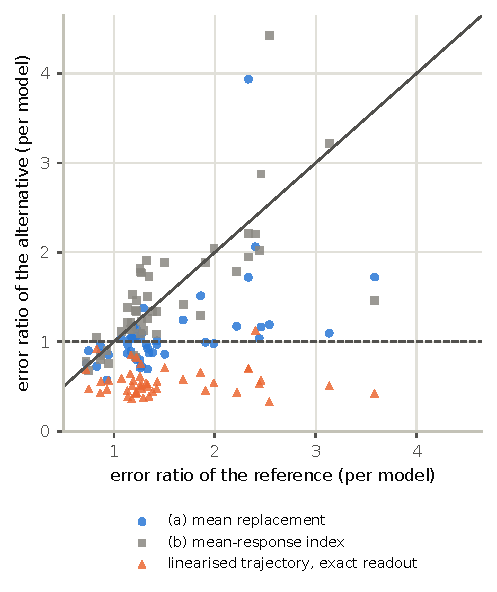
\includegraphics[width=0.56\linewidth]{figures/s2-fig3-per-model.pdf}
\caption{Per-model error ratios at full strength: arm~(a), arm~(b) and the exact readout on the linearised trajectory, against the reference. Solid line: equal error ratios; dashed line: predicting zero change.}
\label{fig:models}
\end{figure}

\subsection{The nonlinearity is in the readout}
\label{sec:mechanism}

\begin{table}[t]
\centering
\caption{Where the nonlinearity lies (silencing, peak index, full strength). Share of error removed: $1-\mathrm{MAE}/\mathrm{MAE}_{\text{first order}}$ per model. Against zero change: mean absolute error minus that of predicting zero change. Means over \NConfModels{} models with 95\% bootstrap intervals.}
\label{tab:mechanism}
\footnotesize
\setlength{\tabcolsep}{3pt}
\begin{tabularx}{\linewidth}{@{}Ylllr@{}}
\toprule
Estimator & Error ratio & Share of error removed & Against zero change & Wrong signs \\
\midrule
\tableinput{generated/s2-table-mechanism.tex}
\bottomrule
\end{tabularx}
\end{table}

\enlargethispage{\baselineskip}\Cref{tab:mechanism} gives the estimators of \cref{sec:counterfactual}. Applying the linearised readout to the exactly simulated trajectories does not help: its error ratio is \RatioCfNetFull{} \RatioCICfNetFull{}, and it removes \RecNetZPFull\% of the first-order error, that is, it adds error. Applying the exact readout to the linearised trajectory removes \RecReadZPFull\%: its error ratio is \RatioCfReadFull{} \RatioCICfReadFull{}, below 1 in \BelowOneCfRead{} of \NConfModels{} models, it beats predicting zero change (difference \MaeDiffCfReadFull{}, \MaeDiffCICfReadFull{}), and only \WrongCfReadFull\% of large effects get the wrong sign. The readout's nonlinearity, not the network's, accounts for Study 1's error (difference in error removed \ReadMinusNetZPFull{}, \ReadMinusNetCIZPFull{}). \Cref{fig:s2-scatter} shows the difference case by case. The same holds for the mean-response index (\RecReadZMFull\% against \RecNetZMFull\%) and under mean replacement (\RecReadMPFull\% against \RecNetMPFull\%; \cref{app:tables}).

The network's trajectories are themselves not linear: the linear approximation misses \TraceLinZero\% of the change in the readout traces (median per model), and adding the second derivative reduces this only to \TraceQuadZero\% (median ratio of the two errors \TraceRatioZero{}). These errors matter much less than the readout's because the index turns each trace into one response and then divides.

\begin{figure}[t]
\centering
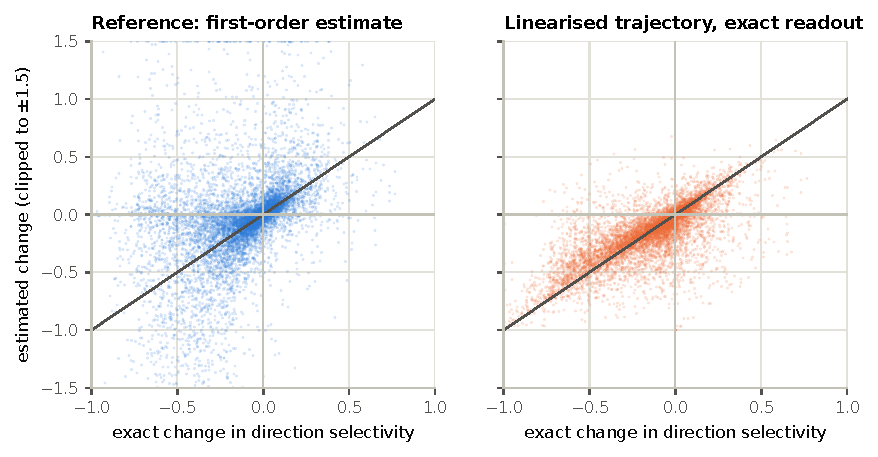
\includegraphics[width=\linewidth]{figures/s2-fig2-predicted-vs-exact.pdf}
\caption{Estimated against exact change in direction selectivity for all \PostCases{} scored silencing cases of the confirmation models at full strength (post hoc case file). Left: the reference, the estimates of \cref{fig:s1-scatter}b. Right: the exact readout applied to the linearised trajectory. Estimates are clipped to $\pm1.5$ for display; the line marks equality.}
\label{fig:s2-scatter}
\end{figure}

\subsection{Within the readout, the ratio}
\label{sec:split}

The split of Amendment~1 separates the two stages of the readout on the linearised trajectory (\cref{tab:mechanism}, green in \cref{fig:ratios}). Applying the exact ratio to the floored linear responses removes \RecRatioZPFull\% of the first-order error: its error ratio is \RatioSplitRatioFull{} \RatioCISplitRatioFull{}, below 1 in \BelowOneSplitRatio{} of \NConfModels{} models, and it beats predicting zero change (\MaeDiffSplitRatioFull{}, \MaeDiffCISplitRatioFull{}). Making only the responses exact and linearising the ratio makes the estimate far worse (error ratio \RatioSplitRespFull{} \RatioCISplitRespFull{}): a linearised ratio applied to large changes of the responses overshoots, as the second-order term does. The ratio stage dominates (difference in error removed \RatioMinusRespZPFull{}, \RatioMinusRespCIZPFull{}). With the mean-response index, whose response stage is the rectification alone, the pattern is the same (\RecRatioZMFull\% removed by the exact ratio against \RecRespZMFull\% by exact responses). The two stages interact strongly: making both exact removes more than the two single changes added together (\InteractionZPFull{}, \InteractionCIZPFull{}), so neither stage alone accounts for the whole effect.

\subsection{Why the second-order estimate overshoots}
\label{sec:second}

This subsection is post hoc. Splitting the second-order term of \cref{eq:second} into the network's part, $\tfrac12 s^2\,\nabla F\cdot K$, and the readout's curvature, $\tfrac12 s^2\,J^{\top}(\nabla^2F)J$, the readout's part makes up \PostShareReadout\% of the term's absolute size (mean over models). The term is concentrated in the cases where the linearised trajectory changes the index's denominator by more than its own size: these are \PostLargeDenFrac\% of cases but carry \PostLargeDenShare\% of the term. The Taylor series of a ratio in the strength converges only while the denominator's change stays below the denominator itself, so in these cases the second-order term diverges. Their mean absolute error is \PostLargeSecond{} for the second-order estimate, \PostLargeFirst{} for the first-order estimate and \PostLargeZero{} for predicting zero change. In the remaining cases the first-order estimate is about as good as predicting zero change (\PostRestFirst{} against \PostRestZero{}), and the second-order estimate is worse (\PostRestSecond{}); it beats the first-order estimate in \PostRestSecondBelowFirst{} of \NConfModels{} models. The curvature available to a second-order correction therefore does not repair the estimate anywhere in these models, and Study 1's failure lies mostly in the cases where silencing changes the response by a large fraction.

\subsection{Strength}
\label{sec:s2-strength}

In the development models (\cref{tab:s2-development}), the reference's error ratio rises from \DevRefPointOne{} at strength 0.1 to \DevRefFull{} at full silencing and passes 1 between strengths 0.25 and 0.5, as Study 1's errors do (\cref{fig:s1-strength}). Under mean replacement it stays below 1 up to strength 0.75 (\DevAThreeQ{}). The exact readout on the linearised trajectory stays below 1 at every strength (\DevCfReadPointOne{} to \DevCfReadFull{}), and the second-order estimate is worse than the first-order one at every strength. In the confirmation models at half strength, the reference's error ratio is \RatioRefHalf{} \RatioCIRefHalf{} and the exact readout on the linearised trajectory reaches \RatioCfReadHalf{} \RatioCICfReadHalf{}.

\subsection{Baseline mismatch}
\label{sec:mismatch}

Using the silencing derivative to estimate the effects of mean replacement gives an error ratio of \RatioMisMeanFull{} \RatioCIMisMeanFull{}, \MisMeanMinusMatchedFull{} \MisMeanMinusMatchedCIFull{} above the matched estimate, and it loses its advantage in screening: its top-10 precision, \TopTenMisMeanFull{}, equals that of anatomy (\AnatMisMeanFull{}; difference \MisMeanTopAnatFull{}, \MisMeanTopAnatCIFull{}). In the other direction, the derivative of mean replacement estimates the effects of silencing with an error ratio of \RatioMisZeroFull{} \RatioCIMisZeroFull{}, lower than the silencing derivative's own (difference \MisZeroMinusRefFull{}, \MisZeroMinusRefCIFull{}).

\subsection{The predictions}
\label{sec:predictions}

Of the \PredPrimaryTotal{} predictions hashed before the development phase, \PredPrimaryHeld{} hold (\cref{app:predictions}). The failures are the size of arm~(c)'s failure (error ratio and wrong-sign rate far above the predicted ranges, and its bias beyond the predicted bound), arm~(a)'s wrong-sign rate (higher than predicted), and the expectation that the mismatched silencing derivative would keep its screening advantage. Of the \PredAddendumTotal{} predictions informed by the development results, \PredAddendumHeld{} hold; the exception is that arm~(b) was predicted to be worse than the reference and is not detectably different.

%======================================================================
\section{Computational cost}
\label{sec:cost}

Per model and for both stimuli, exact silencing of the \SimulatedTypes{} cell types with a path to the readouts took \TimeExactFull{}~s at one strength and \TimeExactBoth{}~s at both strengths, and Study 1's first-order estimates for the eight readouts took \TimeGradient{}~s: \TimeForward{}~s for the forward pass and \TimeBackwardEach{}~s for each readout's backward pass. Exact silencing at one strength was thus slightly faster (model-mean time ratio \TimeRatioFull{}), and at two strengths it took \TimeRatioBoth{} times as long. The two costs scale with different quantities. Exact silencing costs one simulation per intervention, about \TimePerType{}~s per cell type and strength here. The first-order estimate costs one backward pass per readout, about as much as \BackwardOverType{} silencing simulations, and serves every strength at once. It saves computation only when the interventions of interest outnumber the readouts by more than this factor; with \SimulatedTypes{} cell types and eight readouts, the FlyVis models are close to the break-even point. These timings cover the simulation and differentiation on one 6 GB NVIDIA GPU (single precision, \BatchSize{} silencing simulations per batch) and exclude model loading, adaptation to the grey screen and file input and output.

Study 2's forward recursions for the first and second derivatives of all \NSimTypes{} cell types took \TimeTangentsZero{}~s per model on the GPU, \TimeRatioTangents{} times as long as exact silencing of all of them at one strength. Exact mean replacement took \TimeRatioExactMean{} times as long as exact silencing. Study 2 also prespecified a practical rule: screen with Study 1's derivatives, simulate the \FlagBudgetPrimary{} cell types with the largest estimates for each stimulus, and predict zero change for the rest. It removes \FlagRecTenZero\% of the error of predicting zero change in \FlagSecTenZero{}~s per model. That is \FlagPerSecTenZero{} of the error per second, against \ExhaustivePerSec{} per second for simulating every cell type, so the rule never pays in these models at any of the budgets tried (\cref{app:tables}).
